Theory here, in present tense.

This is an equation
\begin{align} \label{theo:eq:newton2}
    F = ma.
\end{align}

We cite our sources like this~\citep{Project1}.

\subsection{Principal Component Analysis (PCA)}

    \subsubsection{Motivation and assumptions}
        Consider the collection of data $X$ which is a $(n\cross m)$ matrix, with $n$ data points, and $m$ features. We might find ourselves in a situation where some features are highly correlated. As a result, some features might be considered obsolete since the trend they describe can easily be described by other features, or combinations of other features. If this is the case, then $X$ contains more features than is strictly necessary in order to explain the trends in the data. Principal component analysis is a technique where we make linear combinations of the original features in such a way that we can describe the data with as few as possible of these new features, effectively reducing the dimensionality of the problem, without loosing too much information about the data itself. By doing this we can perform the computations with a dataset of fewer dimensions, increasing the computational efficiency. We assume that we can describe the data by its variance only. This implies that the mean must be zero, i.e. the data must be in mean-deviation form. We also assume the data to be normally distributed, as a mean-centred normal distribution is the only distribution described by its variance alone.
        
        \begin{figure}
            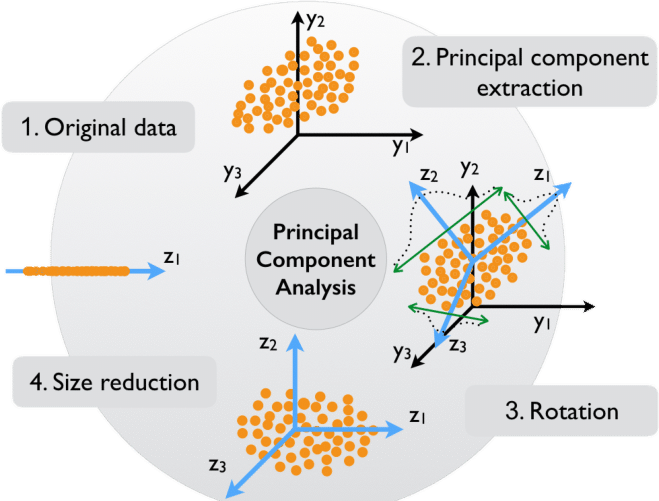
\includegraphics[width=\linewidth]{figs/pca_schematic.png}
            \caption{Schematic representation of PCA. New axes, represented as $z$ in the figure are generated, forming a new basis and a new hyperplane onto which we project the data in order to maximise variance and minimise covariance.\citep{pca_img}}
            \label{theo:fig:pca_schematic}
        \end{figure}
        
        From a geometrical point of view, this can be thought of as expressing the data in a different coordinate system, and PCA involves determining these new axes. Figure \ref{theo:fig:pca_schematic}  shows a visual interpretation of this, where the black axes are the original ones, and we find the new blue axes with PCA. These are determined in such a way that the variance of the data is maximised in the new coordinate system, while minimising the covariance between features. We must impose this criterion since we want as few new features as possible, hence we do not want them to co-vary, but rather vary as much as possible. 

    \subsubsection{Mathematical consideration}

    Our goal is to reduce the dimensionality of the data, thus we want to represent the data as a matrix $Y$ with shape $(n\cross d)$ where $d\leq m$. This indicates that we are after a linear transformation $T:\mathbb{R}^{n\cross m} \to \mathbb{R}^{n\cross d}$ which we can define by $T(X) = XP = Y$, where $P$ is an orthonormal matrix of shape $m\cross d$, which we intend to find. $P$ must fulfil our criterion on $Y$, which is high variance and low covariance. This can be done by diagonalising the covariance matrix of $Y$ given by:

    \begin{align}\label{theo:eq:Y_covariance}
        S_Y &= n_cY^TY\nonumber\\
        &= n_c(XP)^T(XP) \nonumber\\
        &= n_cP^T(X^TX)P,
    \end{align} 
    where $n_c = 1/(n-1)$ is the normalisation due to $n$ data points.

    With \citep[ch. 5.3]{linalgbok} we can show that any square symmetric matrix, like $X^TX$, can be expressed as $EDE^T$ where the columns of $E$ are the orthonormal eigenvectors of $X^TX$, and $D$ is a diagonal matrix. Inserting this into equation  \ref{theo:eq:Y_covariance} we obtain that $S_Y = n_cP^TEDE^TP$. We see that $P=E \implies S_Y=n_c D$\footnotemark, since $P$ is then orthonormal and thus $P^T=P^{-1}$.

    \footnotetext{This is not necessarily trivial since we want $P$ to have shape $(m\cross d)$. $E$ contains all the eigenvectors of $X^TX$ and has thus shape $(m\cross m)$. This is easily surpassed by setting $d=m$ while showing this, and then reduce the dimension of $P$ when we need it later. We also note that this works mathematically if we let $E$ contain the $d$ eigenvectors of $X^TX$ with the largest eigenvalues. Then $D$ must be a $(d\cross d)$ diagonal matrix, which is of similar shape as $S_Y$.}

    Hence, choosing the columns of $P$ to be the orthonormal eigenvectors of $X^TX$ yield a diagonal covariance matrix $S_Y$, exactly what we want. This link can also be made through the singular value decomposition (SVD). We can express any matrix $X$ as $X=U\Sigma V^T$ \citep[ch. 7.4]{linalgbok}, where $V$ is a matrix containing the orthonormal eigenvector of $X^TX$. Without delving further into SVD, we see that $P$ may also be found from the column vectors in $V$. 
    
    We conclude that the principal components of $X$ can be expressed as $P=[\vec{p}_1, \dots \vec{p}_d]$, where $\vec{p}_1$ is the eigenvector of $X^TX$ that corresponds to the largest eigenvalue, $\vec{p}_2$ to the second largest and so on. This continues until we have found $d$ principal components. Each $\vec{p}_i$ is by construction a linear combination of the original features and has shape $(m\cross 1)$.   The elements of PCA may then be summarised as follows:

    \begin{enumerate}
        \item Make sure $X$ has shape $(n\cross m)$ and is in mean-deviation form.
        \item Find $P$ either from $V$ or the eigenvectors of $X^TX$ directly.
        \item Calculate $Y=XP$.
        \item Find the diagonal covariance $S_Y=n_cY^TY$.
    \end{enumerate}
    
    \subsubsection{Interpretation}
    Now we have a recipe of finding the principal component $P$, but what do they really mean? We perform PCA in order to reduce the redundancy of features, to express the data with as few features/dimensions as possible without loosing too much information. We therefore make new features that are linear combinations of the original features, but with zero covariance. This means that when we ``choose'' the first principal component $\vec{p}_1$, we find the direction in feature space, along which the variance of the data is maximised. In other words, if we were to project all data points down on a line, $\vec{p}_1$ would be the line that gives the largest variance, i.e. yield as much information about the data as possible for a 1D data set. When finding the next principal component we repeat this process, but restrict ourselves to only ``choosing'' directions in feature space orthogonal to the previous. 
    
    Having $d$ principal components means that we have found $d$ directions in feature space, all with a maximised variance. These can be though of as a new basis or representing our data $X$. Then the matrix $P$ can be interpreted as the change of basis matrix between $X$ and $Y$. $Y$ are the same data points, but expressed in the basis of the principal components. They are the data points projected onto a hyperplane set up by the vectors $\vec{p}_i$. This can also be inferred from figure \ref{theo:fig:pca_schematic}. We also notice a rather neat consequence of the SVD, that finding the principal components of $X$ equates to finding an orthonormal basis that span $\text{Row}(X)$. The $i$-th diagonal element of $S_Y$ is the variance, $\sigma_i^2$ of the data along $\vec{p}_i$. The total variance is the sum over these diagonal elements, or the trace, $\text{tr}(S_Y)$.

     

\subsection{Neural Networks}
    First, it will be wise to take a minute to recap some of the details of how a \textit{feed-forward nerual network} (FFNN) is built and trained from~\cite{Project2}. They are made up of sequential \textit{layers} taking in the input from the previous layer and passing it on to the next one. There will always be an input layer, taking in the features $x$ producing some observation $y$, and an output layer transforming the input from the second to last layer into an appropriate output. In classification problems, the outputs will usually be probabilities between $0$ and $1$ for the input to produce an output in a given category. In regression, the output layer usually transforms the output to be a single number $\tilde{y}$ for the predicted value.

    When passing the output from one layer to the next, a linear transformation is done. Denoting the output vector from layer $\ell$ as $\vec{a}^\ell$, the transformation produces a \textit{response} $\vec{z}^{\ell} = W^\ell \vec{a}^{\ell-1} + \vec{b}^\ell$, where $W^\ell$ is a weight matrix, and $\vec{b}^\ell$ is called the bias. The response vector is then passed through an activation function (which is generally non-linear) to produce the \textit{activation} $\vec{a}^\ell = f(\vec{z}^\ell)$.

\subsection{Local Winner-Takes-All (LWTA)}
    \comment{Explain local learning and sparse pathways -\Anna}
    The idea of LWTA algorithms is to implement local learning in the neural network, such that the entire network does not learn how to transform a given input, but it is rather outsourced to local parts of the network. In LWTA algorithms, sparse pathways learn during training, and these pathways are selected at inference time. The nodes in each layer are grouped into a number of groups $G$, and Winner Takes All is applied on the activation of each of these groups, only passing on the maximal output in the group.

    \subsubsection{Maxout and Channel-Out}
        \comment{Some introductory sentence establishing the excistence of the two algorithms. "There are mainly two algowithms classifying as LWTA; maxout, where pathways are only formed posteriori, and channel-out, where they are also formed anteriori." or something -\Anna}
        The \textit{maxout} activation passes the input from the previous layer through the weight kernel and adds the bias as normal, but then only passes on the activation from the most active node in each group of the layer. Each group then has a common set of weight connections to the next layer in  the network.

        During back propagation in training, the weights of each group are trained according to the activation of the most active node. This can be seen from the gradient of the cost function in the direction of one of the weights of an inactive node: the learning is proportional to $\pd[w^{\ell}_{ij}]{C} \propto \pd[a^\ell_i]{C} = 0$, because any infinitesimal change in the activation would still result in no activation if $a_i$ was not already the maximum of the group.

        \comment{comment on/specify the paths being made due to the weights of the previous layer. See that it is specified below, but I think we could do it here as well. Should be easier when illustrations are included -\Anna}

        % \begin{algorithm}
        %     \caption{Max Out activation}
        %     \begin{algorithmic}[1]
        %         \For{$i=1$ to $g$}
        %             \State $a_i \gets -\infty$
        %             \For{$j=1$ to $n \bmod g$}
        %                 \If{$z_{ij} > a_i$}
        %                     \State $a_i \gets z_{ij}$
        %                 \EndIf
        %             \EndFor
        %         \EndFor
        %     \end{algorithmic}
        % \end{algorithm}

        \textit{Channel-out} makes a subtle, but meaningful, change to the maxout algorithm. Instead of every group having a common set of weight connections to the next layer, every node has its own set of weight connections. This results in not only local learning of the weights during backpropagation, but also leads to the activation winner choosing the set of weights that will be used in the next layer at inference time.
        Effectively, a channel-out layer works the same way as an ordinary dense layer with a linear activation function, but sets all the activations of the nodes that do not win their group to zero before passing them on to the next layer.
        Same as with maxout, only the weights of the active nodes are trained, but this also applies to the next layer, where only weights connected to the active nodes are trained. So the local learning goes both forwards and backwards from a channel-out layer, in contrast to just backwards in the case of maxout.

    \subsection{Neurological Background}
   


    
        
